\section{Approach}
\label{sec:approach}

\begin{figure*}[t]
\centering
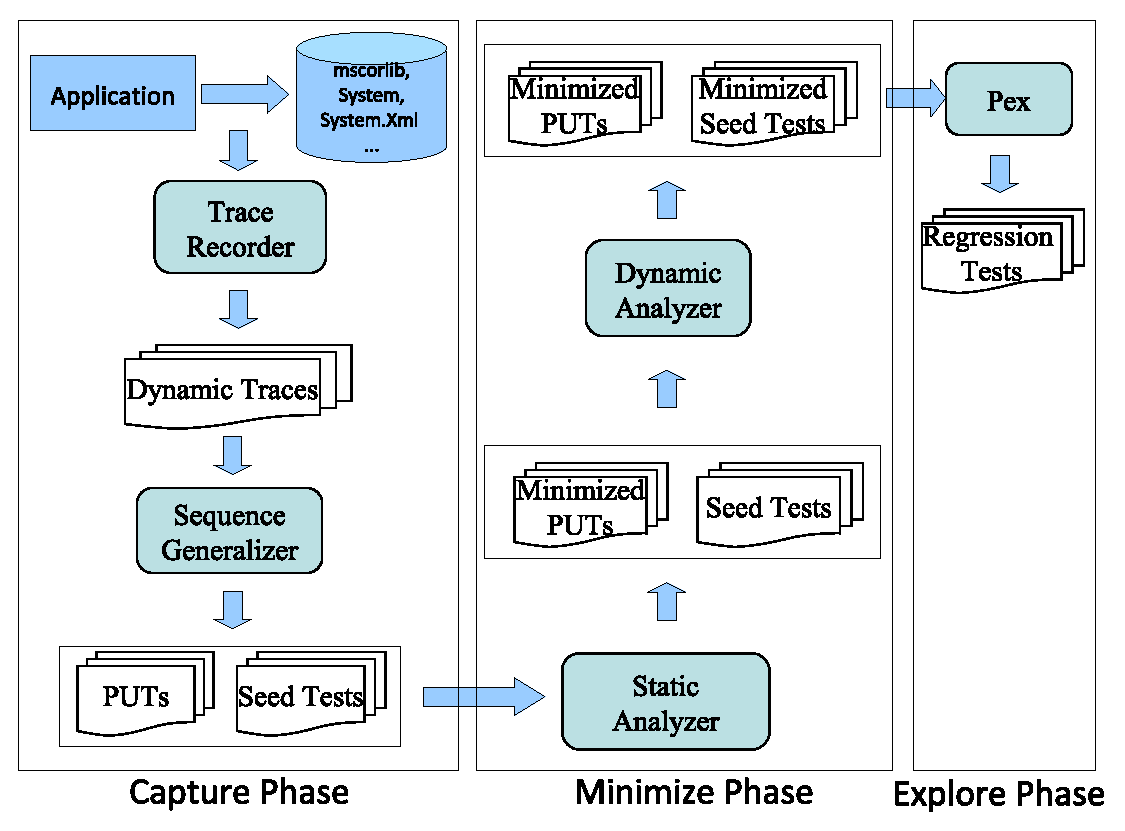
\includegraphics[scale=0.60,clip]{figs/approach1.eps}\vspace*{-2ex}
\caption{A high-level overview of our approach} \label{fig:overview}\vspace*{-3ex}
\end{figure*}

Figure~\ref{fig:overview} shows the high-level overview of our approach. Our approach includes three major phases: \emph{capture}, \emph{minimize}, and \emph{explore}. In the
capture phase, our approach records dynamic traces from program executions. Our approach next transforms these dynamic traces into PUTs and seed tests. Among recorded traces, we identify that there are many duplicate traces since the same sequence of method calls can get invoked multiple times during program executions. Consequently,
the generated PUTs and seed tests also include duplicates. In the minimize phase, we use a combination of static and dynamic analyses to filter out duplicate PUTs and seed tests, respectively. In the explore phase, we use Pex to explore PUTs to generate regression tests that achieve a high coverage of the code under test. We next explain each phase in detail.

%------------------------------------------------------------------------
\subsection{Capture Phase}
\label{sec:capture}

In the capture phase, our approach records dynamic traces from program executions. The capture phase uses a profiler that records method calls invoked by the application during execution. The capture phase records both the method calls invoked and the concrete values passed as arguments to those method calls. Figure~\ref{fig:dynamictrace} shows an example dynamic trace recorded by the capture phase. Statement 2 shows the concrete value ``\CodeIn{<\%\@ Page..$\backslash$u000a}'' passed as an argument for the \CodeIn{Match} method. Our recorded traces are complete and do not require any other primitive values or non-primitive objects.

\begin{figure}[t]
\begin{CodeOut}
01: TagRegex tagex = new TagRegex();\\
02: Match mc = ((Regex)tagex).Match("<\%\@ Page..$\backslash$u000a",108);\\
03: Capture cap = (Capture) mc;\\
04: int indexval = cap.Index;\\
\end{CodeOut}\vspace*{-5ex}
\Caption{\label{fig:dynamictrace} An example dynamic trace recorded by the capture phase.}\vspace*{-3ex}
\end{figure}

Our approach uses a technique similar to Saff et al.~\cite{david:java} for transforming recorded traces into PUTs and seed tests. To generate PUTs, our approach identifies all constant values and promotes those constant values as parameters. Furthermore, our approach identifies return values of method calls in the PUT and promotes those return values as \CodeIn{out} parameters for the PUT. In C\#, these \CodeIn{out} parameters represent the return values of a method. Our approach next generates seed tests that include all concrete values from the dynamic traces. Figure~\ref{fig:putut} shows a PUT and a seed test generated from the dynamic trace shown in Figure~\ref{fig:dynamictrace}.

\begin{figure}[t]
\begin{CodeOut}
\textbf{PUT:}\\
00: public static void $F_1$(string $val_1$, int $val_2$, out int $out_1$)\\
01: \hspace*{0.2in}TagRegex tagex = new TagRegex();\\
02: \hspace*{0.2in}Match mc = ((Regex)tagex).Match($val_1$, $val_2$);\\
03: \hspace*{0.2in}Capture cap = (Capture) mc;\\
04: \hspace*{0.2in}$out_1$ = cap.Index;\\
05: \}\\

\textbf{Seed Test:}\\
06: public static void $T_1$() \{\\
07: \hspace*{0.2in}int index;\\
08: \hspace*{0.2in}$F_1$("<\%@ Page..$\backslash$u000a", 108, out index);\\
09: \}\\
\end{CodeOut}\vspace*{-3ex}
\Caption{\label{fig:putut} A PUT and a seed test generated
from the dynamic trace in Figure~\ref{fig:dynamictrace}.}\vspace*{-3ex}
\end{figure}

The generated PUT includes two parameters and one \CodeIn{out} parameter. The \CodeIn{out} parameter is the return value of the method \CodeIn{Capture.Index}. These \CodeIn{out} parameters are later used to generate test assertions in regression tests (Section~\ref{sec:explore}). The figure also shows a seed test generated from the dynamic trace. 
The seed test includes concrete values of the dynamic trace and invokes the generated PUT with those concrete values.

%------------------------------------------------------------------------
\subsection{Minimize Phase}
\label{sec:minimize}

Our approach records dynamic traces during actual program executions. As the same sequence of method calls can be invoked multiple times during program executions,
we identify that there are many duplicates among recorded dynamic traces. Consequently, there are many duplicates among generated PUTs and seed tests. For example, in our evaluations, we identify that $84$\% of PUTs and $70$\% of seed tests are classified as duplicates by our minimize phase. In the minimize phase, our approach filters out duplicate PUTs and seed tests. The primary reason for filtering out duplicates is that exploration of duplicate PUTs is redundant and can also lead to scalability issues while generating regression tests.

We use PUTs and seed tests shown in Figure~\ref{fig:samplePutAndUT} as illustrative examples. The figure shows a method under test \CodeIn{foo}, two PUTs, and three seed tests. We use these examples primarily for explaining our minimize phase and our actual PUTs and seed tests are much more complex than these illustrative examples. We first present our criteria for a duplicate PUT and a seed test and next explain how we filter out such duplicate PUTs and seed tests.

\textbf{Duplicate PUT:} We consider a PUT, say $P_1$, as a duplicate of another PUT, say $P_2$, if both $P_1$ and $P_2$ have the same sequence of Microsoft Intermediate Language (MSIL)\footnote{\url{http://msdn.microsoft.com/en-us/library/c5tkafs1(VS.71).aspx}} instructions.

\textbf{Duplicate Seed Test:} We consider a seed test, say $S_1$, as a duplicate of another seed test, say $S_2$, if both $S_1$ and $S_2$ exercise the same execution path.
This execution path refers to the path that starts from the beginning of PUT and goes through all (transitive) method calls.

\begin{figure}[t]
\begin{CodeOut}
00:Class A \{\\
01:\hspace*{0.2in}public void foo(int arg1, int arg2, int arg3) \{\\
02:\hspace*{0.4in}if (arg1 > 0)\\
03:\hspace*{0.6in}Console.WriteLine("arg1 > 0"); \\
04:\hspace*{0.4in}else\\
05:\hspace*{0.6in}Console.WriteLine("arg1 <= 0"); \\
06:\hspace*{0.4in}if (arg2 > 0)\\
07:\hspace*{0.6in}Console.WriteLine("arg2 > 0"); \\
08:\hspace*{0.4in}else\\
09:\hspace*{0.6in}Console.WriteLine("arg2 <= 0"); \\
10:\hspace*{0.4in}for (int c = 1; c <= arg3; c++)  \{ \\
11:\hspace*{0.6in}Console.WriteLine("loop") \\
12:\hspace*{0.4in}\}\\
13:\hspace*{0.2in}\}\\
14:\}\\
\\
15:void PUT1(int arg1, int arg2, int arg3) \{\\
16:\hspace*{0.2in}A a = new A();\\
17:\hspace*{0.2in}a.foo(arg1, arg2, arg3);\\
18:\}\\
\\
19:public void SeedTest1() \{\\
20:\hspace*{0.2in}PUT1(1, 1, 1);\\
21:\}\\
\\
22:void PUT2(int arg1, int arg2, int arg3) \{\\
23:\hspace*{0.2in}A a = new A();\\
24:\hspace*{0.2in}a.foo(arg1, arg2, arg3);\\
25:\}\\
\\
26:public void SeedTest2() \{\\
27:\hspace*{0.2in}PUT2(1, 10, 1);\\
28:\}\\
\\
29:public void SeedTest3() \{\\
30:\hspace*{0.2in}PUT1(5, 8, 2);\\
31:\}\\
\end{CodeOut}\vspace*{-2ex}
\caption{\label{fig:samplePutAndUT}Two PUTs and associated seed tests generated by the capture phase.}\vspace*{-3ex}
\end{figure}

Our approach uses static analysis to identify duplicate PUTs. For example, our approach compares the method bodies of \CodeIn{PUT1} and \CodeIn{PUT2} at the level of MSIL instructions. In this example, our approach considers \CodeIn{PUT2} as a duplicate of \CodeIn{PUT1} as both the PUTs include the same sequence of MSIL instructions. As \CodeIn{PUT2} is a duplicate of \CodeIn{PUT1}, our approach automatically replaces the \CodeIn{PUT2} method call in \CodeIn{SeedTest2} with \CodeIn{PUT1}.

After filtering out duplicate PUTs, our approach uses dynamic analysis for filtering out duplicate seed tests. To identify duplicate seed tests, our approach executes each seed test and monitors its execution path in the code under test. For example, \CodeIn{SeedTest1} follows the path ``3 $\rightarrow$ 7 $\rightarrow$ 11'' in \CodeIn{PUT1}. Our approach considers \CodeIn{SeedTest2} as a duplicate of \CodeIn{SeedTest1}, as \CodeIn{SeedTest2} also follows the same path ``3 $\rightarrow$ 7 $\rightarrow$ 11'' in \CodeIn{PUT1}. Consider another unit test \CodeIn{SeedTest3} shown in Figure~\ref{fig:samplePutAndUT}. Our approach does not consider \CodeIn{SeedTest3} as a duplicate of \CodeIn{SeedTest1} as \CodeIn{SeedTest3} follows the path ``3 $\rightarrow$ 7 $\rightarrow$ 11 $\rightarrow$ 11'', since \CodeIn{SeedTest3} iterates the loop in Statement 10 two times.

%------------------------------------------------------------------------
\subsection{Explore Phase}
\label{sec:explore}

In the explore phase, our approach uses Pex to generate regression tests from PUTs. Although seed tests generated in the capture phase can be considered as regression tests, most seed tests tend to exercise common happy paths such as paths that do not include error-handling code in the code under test. In only few rare scenarios, seed tests may exercise the paths related to error-handling code, if such scenarios happen during program executions. Therefore, these seed tests do not achieve high coverage of the corner cases and error handling of the code under test.

To address this issue, we use Pex to explore generated PUTs. Inspired by Patrice et al.~\cite{patrice08:whitebox}, we use seed tests to assist Pex during exploration of PUTs. Using seed tests increases the effectiveness of Pex or any other dynamic-symbolic-execution-based approach in two major ways. First, with seed tests, Pex executes those seed tests and internally builds an execution tree with the paths covered by the seed tests. Pex starts exploration with this pre-populated tree and extends this tree by \emph{flipping} individual branch nodes via constraint solving. On the other hand, without any seed tests, Pex starts exploration with an empty execution tree. Therefore, using seed tests significantly reduce the amount of time required in generating tests from PUTs. Second, seed tests can help cover certain paths that are hard to be covered without using those tests. For example, it is quite challenging for Pex or any other dynamic-symbolic-execution-based approach to generate concrete values for variables
that require complex values such as IP addresses, URLs, doubles. In such scenarios, seed tests can help provide desired concrete values to cover those paths.

Pex generated $86$ regression tests for the PUT shown in Figure~\ref{fig:putut}. Figure~\ref{fig:generatedtests} shows three sample regression tests generated by Pex. In regression tests 1 and 2, Pex automatically annotated the unit tests with the expected exceptions \CodeIn{ArgumentNullException} and \CodeIn{ArgumentOutOfRangeException}, respectively. Since the PUT (Figure~\ref{fig:putut}) includes an \CodeIn{out} parameter, Pex generated assertions in regression tests based on actual values captured while 
generating the test. These expected exceptions or assertions serve as test oracles in regression tests.

\begin{figure}[t]
\begin{CodeOut}
\textbf{Regression Test 1:}\\
00: [PexRaisedException(typeof(ArgumentNullException))]\\
01: public static void $F_{102}$() \{\\
02: \hspace*{0.2in}int i = default(int); \\
03: \hspace*{0.2in}$F_1$ ((string)null, 0, out i);\\
04: \}\\
\\
\textbf{Regression Test 2:}\\
00: [PexRaisedException(typeof(ArgumentOutOfRangeException))]\\
01: public static void $F_{110}$() \{\\
02: \hspace*{0.2in}int i = default(int);\\
03: \hspace*{0.2in}$F_1$("", 1, out i);\\
04: \}\\
\\
\textbf{Regression Test 3:}\\
00: public static void $F_{103}$() \{\\
01: \hspace*{0.2in}int i = default(int);\\
02: \hspace*{0.2in}$F_1$ ("$\backslash$0$\backslash$0$\backslash$0$\backslash$0$\backslash$0$\backslash$0$\backslash$0<$\backslash$u013b$\backslash$0", 7, out i); \\
03: \hspace*{0.2in}PexAssert.AreEqual<int>(0, i);\\
04: \}\\
\\
\end{CodeOut}\vspace*{-5ex}
\Caption{\label{fig:generatedtests} Regression tests generated by Pex by exploring 
the PUT shown in Figure~\ref{fig:putut}.}\vspace*{-1ex}
\end{figure}

Although Pex is effective in exploring PUTs and generating unit tests, we identify that Pex or any other dynamic-symbolic-execution-based approaches can take a long time (days or months) to explore generated PUTs with dynamic symbolic execution on a single machine. To address this issue, our approach uses an enhanced distributed setup originally proposed in our previous work~\cite{tillman:pexwhite}. Our distributed setup allows to launch multiple Pex processes on several machines. Once started, our distributed setup is designed to run forever in iterations. The primary reason for such a setup is that it is hard to decide when to stop exploring a PUT. For example, loops in the code under test introduce infinite number of possible paths and it will take infinite amount of time to generate tests that cover all possible paths.

To address the preceding issue, we explore PUTs in iterations bounded by various parameters. For example, consider a timeout parameter that describes when to stop exploring a PUT. In the first iteration, we set three minutes for the timeout parameter. This timeout parameter indicates that we terminate exploration of a PUT after three minutes. In the first iteration, we explore all PUTs with these bounded parameters. In the second iteration, we double the values of these parameters. For example, we set six minutes for the timeout parameter in the second iteration. Doubling the parameters gives more time for Pex in exploring new paths in the code under test. To avoid Pex exploring the same paths that were explored in previous iterations, we maintain a pool of all generated tests. We use the tests in the pool generated by previous iterations as a seed for further iterations. For example, tests generated in Iteration 1 are used as seed tests in Iteration 2. Based on the amount of time available for generating tests, tests can be generated in further iterations.
